%%%%%%%%%%%%%%%%%%%%%%%%%%%%%%%%%%%%%%%%%%%%%%%%
%% Compile the master file!
%% 		Slides: Antonio Machicao y Priemer
%% 		Course: GK Linguistik
%%%%%%%%%%%%%%%%%%%%%%%%%%%%%%%%%%%%%%%%%%%%%%%%

%%%%%%%%%%%%%%%%%%%%%%%%%%%%%%%%%%%%%%%%%%%%%%%%%%%%
%%%             Metadata                         
%%%%%%%%%%%%%%%%%%%%%%%%%%%%%%%%%%%%%%%%%%%%%%%%%%%%      

\title{Grundkurs Linguistik}

\subtitle{Syntax II: Einführung \& Terminologie}

\author[A. Machicao y Priemer]{
	{\small Antonio Machicao y Priemer}
	\\
	{\footnotesize \url{http://www.linguistik.hu-berlin.de/staff/amyp}}
%	\\
%	\href{mailto:mapriema@hu-berlin.de}{mapriema@hu-berlin.de}}
}

\institute{Institut für deutsche Sprache und Linguistik}

%\date{ }

%\publishers{\textbf{6. linguistischer Methodenworkshop \\ Humboldt-Universität zu Berlin}}

%\hyphenation{nobreak}


%%%%%%%%%%%%%%%%%%%%%%%%%%%%%%%%%%%%%%%%%%%%%%%%%%%%
%%%             Preamble's End                  
%%%%%%%%%%%%%%%%%%%%%%%%%%%%%%%%%%%%%%%%%%%%%%%%%%%%      


%%%%%%%%%%%%%%%%%%%%%%%%%      
\huberlintitlepage[22pt]

\iftoggle{toc}{
\frame{
\begin{multicols}{2}
	\frametitle{Inhaltsverzeichnis}\tableofcontents
	%[pausesections]
\end{multicols}
	}
	}


%%%%%%%%%%%%%%%%%%%%%%%%%%%%%%%%%%
%%%%%%%%%%%%%%%%%%%%%%%%%%%%%%%%%%
%%%%%LITERATURE:

%% Allgemein
\nocite{Glueck&Roedel16a}
\nocite{Grewendorf&Co91a} 
\nocite{Luedeling2009a} 
\nocite{Meibauer&Co07a} 
\nocite{Repp&Co15a} 

%% Morphologie
%\nocite{Eisenberg04}

%% Syntax
\nocite{Adger04a}
%\nocite{Altmann&Hofmann08a} % Satztypen & Satzmodi
%\nocite{Altmann93a} % Satztypen & Satzmodi
\nocite{Brandt&Co06a} 
\nocite{Fries&MyP16b} % Akzeptabilität
\nocite{Fries16a} % Grammatikalität
\nocite{Fries&MyP16d} % Kompetenz vs Performanz
\nocite{Fries&MyP16c} % GG
\nocite{Fries&MyP16a} % X-Bar-Theorie
%\nocite{Fries16e} % Satztyp
%\nocite{Fries16d} % Satzmodus 
\nocite{Grewendorf&Co91a} 
\nocite{MyP17b} % Kerngrammatik
\nocite{MyP18a} % Konstituententest
\nocite{MyP18b} % Kopf
\nocite{MyP18c} % Phrase
\nocite{MyP18g} %Entscheidungsfragesatz
\nocite{MyP18i} %Ergänzungsfragesatz
\nocite{MuellerS13f} 
\nocite{MuellerS15b}
\nocite{Stechow&Sternefeld88a}
%\nocite{Sternefeld06a}
%\nocite{Sternefeld06b}
%\nocite{Woellstein10a} % Topologisches Feldermodell

%%%%%%%%%%%%%%%%%%%%%%%%%%%%%%%%%%

\begin{frame}
	\frametitle{Begleitlektüre}
		\begin{itemize}
			\item \textbf{obligatorisch:}
				\begin{itemize}
					\item[] \citet{MyP18a}
				\end{itemize}
			\end{itemize}
		
			\begin{block}{Lektüre für die vorlesungsfreie Zeit}
			\begin{itemize}
				\item \textbf{obligatorisch:}	
				\begin{itemize}	
					\item[] \citet{Woellstein10a}: Kapitel 2 \& 3 (S. 20--53)
					\item[] \citet{MyP18c}
				\end{itemize}
				\item \textbf{optional:}
					\begin{itemize}
						\item[] \citet{Brandt&Co06a}: Kapitel 5--9 (S. 26--65)
					\end{itemize}	
				\end{itemize}
		\end{block}
	
\end{frame}

%%%%%%%%%%%%%%%%%%%%%%%%%%%%%%%%%%
\section{Syntax II: Einführung und Terminologie}

%%%%%%%%%%%%%%%%%%%%%%%%%%%%%%%%%%
\subsection{Was bisher geschah \dots }

\iftoggle{sectoc}{
	\frame{
		%\begin{multicols}{2}
		\frametitle{~}
		\tableofcontents[currentsubsection,subsubsectionstyle=hide]
		%\end{multicols}
	}
}


%%%%%%%%%%%%%%%%%%%%%%%%%%%%%%%%%%
\begin{frame}
\frametitle{Was bisher geschah \dots }

%\begin{itemize}
%	\item 
	Sie wissen bereits:
	
	\begin{itemize}
		\item \textbf{womit} sich die Syntax befasst,
		\item wie man Syntax \textbf{definieren} kann,
		\item dass man auch \textbf{Konstituenten} und \textbf{Kategorien} einbeziehen muss,
		\item dass \textbf{Linearität} $\neq$ \textbf{Struktur},
		\item was der Unterschied zwischen \textbf{Grammatikalität} und \textbf{Akzeptabilität} ist,
		\item was der Unterschied zwischen \textbf{deskriptiv} und \textbf{präskriptiv} ist.
	\end{itemize}
%\end{itemize}

\end{frame}


%%%%%%%%%%%%%%%%%%%%%%%%%%%%%%%%%%
%%%%%%%%%%%%%%%%%%%%%%%%%%%%%%%%%%
\subsection{Generative Grammatik}

\iftoggle{sectoc}{
	\frame{
		%\begin{multicols}{2}
		\frametitle{~}
		\tableofcontents[currentsubsection,subsubsectionstyle=hide]
		%\end{multicols}
	}
}


%%%%%%%%%%%%%%%%%%%%%%%%%%%%%%%%%%
\begin{frame}
\frametitle{Generative Grammatik}

\begin{minipage}[c]{0.57\textwidth}
\begin{itemize}
	\item<1-> Wie gelangen wir zu den deskriptiven Regeln, um die (Un-)Grammatikalität innerhalb eines Regelapparats zu modellieren?

%\pause

	\medskip
	\item<2->  \textbf{Sprachliche Intuition}: \textbf{Sprecher} haben ein \textbf{Gefühl} dafür, was sie in ihrer Muttersprache sagen können und was nicht.
	
	Durch \textbf{Introspektion} (Selbstbefragung) gelangen sie zu diesem Wissen. Dadurch befragen sie ihre sog.\ \textbf{muttersprachliche Kompetenz}.
	
%\pause
	
	\medskip 
	\item<3-> Sprachliche Intuition: wesentlich in den sog.\ generativen Syntaxtheorien seit \citet{Chomsky57x}
	

\end{itemize}
\end{minipage}
%%
%%
\begin{minipage}[c]{0.40\textwidth}

\begin{figure}
	\centering
\only<1->{	
	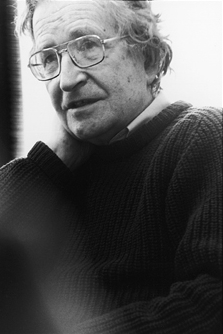
\includegraphics[scale=.5]{material/chomsky01}\label{Abb1}
}
\end{figure}

\end{minipage}

\end{frame}


%%%%%%%%%%%%%%%%%%%%%%%%%%%%%%%%%%
%\begin{frame}
%\frametitle{Generative Grammatik}
%
%\begin{itemize}
%
%	\item Sprachliche Intuition \ras wesentlich in den sog. generativen Syntaxtheorien seit \citet{Chomsky57x}
%
%\begin{figure}
%\centering
%	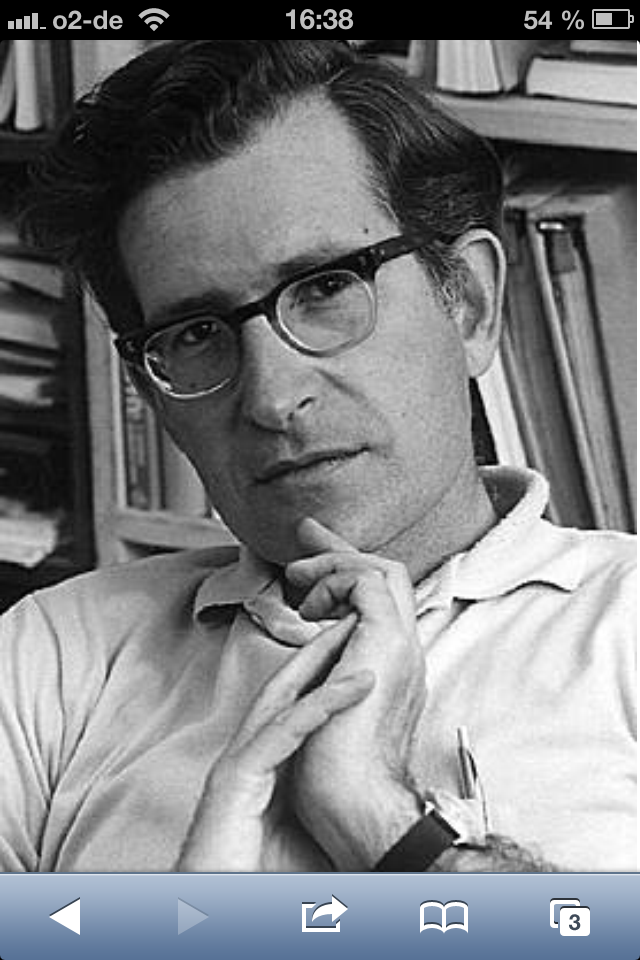
\includegraphics[scale=.17]{material/03chomsky}
%\end{figure}
%
%	
%\end{itemize}
%
%\end{frame}


%%%%%%%%%%%%%%%%%%%%%%%%%%%%%%%%%%
%\begin{frame}
%\frametitle{Generative Grammatik}


%\begin{itemize}
	
%	\item Sprachliche Intuition: wesentlich in den sog.\ generativen Syntaxtheorien seit \citet{Chomsky57x}
		
%\end{itemize}


%\begin{figure}
%	\centering
%	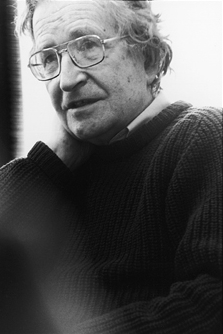
\includegraphics[scale=.5]{material/chomsky01}\label{Abb1}
%\end{figure}

%\end{frame}


%%%%%%%%%%%%%%%%%%%%%%%%%%%%%%%%%%
\begin{frame}
\frametitle{Generative Grammatik}

\begin{itemize}
	\item Was ist diese Generative Grammatik (GG)? 
	\medskip
	\item Seit \citet{Chomsky57x} und \citet{Chomsky65a}
	\medskip
	\item \textbf{dynamische Theorie} (vgl.\ statische Theorie \ras \zB Strukturalismus)
	\begin{itemize}
		\item Grammatik als dynamisches System: Regelsystem, das wohlgeformte Strukturen \emph{erzeugt}
		\medskip
		\item Strukturalistisches Konzept \gqq{Langue} setzt ein statisches Zeichensystem voraus. 
	\end{itemize}

\end{itemize}

\end{frame}


%%%%%%%%%%%%%%%%%%%%%%%%%%%%%%%%%%
\begin{frame}
\frametitle{Generative Grammatik}

\begin{itemize}
	\item Klare Definition des Untersuchungsgegenstandes \gqq{Sprache}:
	\begin{itemize}
		\item Keine Beschreibung mehr von \gqq{sprachlichen} Phänomenen, ohne davor den Begriff \gqq{Sprache} zu definieren / einzuschränken.
		\medskip
		\item \textbf{I-Language} \ras intrinsische Kompetenz des idealen Sprecher"=Hörers (Trennung zwischen Kompetenz und Performanz)
	\end{itemize}
	\medskip
	\item Linguistik als Wissenschaft \ras durch Formalisierung
	\medskip
	\item \textbf{Rationalistische} Vorgehensweise (Cartesianische Linguistik)
	\begin{itemize}
		\item Bruch mit behavioristischer Vorgehensweise (Empirismus)
		\item Rationalistische Sichtweise des Spracherwerbs
		\item Universalgrammatik \ras genetisch verankerte Grundlage der menschlichen Sprachfähigkeit
	\end{itemize}
\end{itemize}

\nocite{Fries&MyP16d}

\end{frame}


%%%%%%%%%%%%%%%%%%%%%%%%%%%%%%%%%%
\begin{frame}
\frametitle{Generative Grammatik}

\begin{itemize}
	\item Verwandtschaft zwischen Sätzen erkennen, beschreiben und erklären (Erklärungsadäquatheit) \ras Transformationen
	
	\eal 
	\ex Man kauft Bier.
	\ex Bier wird gekauft.
	\zl
	
	\medskip	
	\item Beschreibung von sprachlichen Phänomenen ist nicht das primäre Ziel.
\end{itemize}

\end{frame}


%%%%%%%%%%%%%%%%%%%%%%%%%%%%%%%%%%
\begin{frame}
\frametitle{Generative Grammatik}

\begin{block}{Ziel generativer Theorien}
Durch eine \textbf{deskriptive} Vorgehensweise wird ein Regelapparat erstellt, um \textbf{lineare} und \textbf{hierarchische} Gesetzmäßigkeiten des Satzbaus zu \textbf{beschreiben}. Daraus wird versucht, allgemeine (\textbf{universelle}) Gesetzmäßigkeiten der menschlichen Sprachfähigkeit abzuleiten, um somit die menschliche (Sprach)\textbf{Kompetenz zu erklären}.
\end{block}

\end{frame}


%%%%%%%%%%%%%%%%%%%%%%%%%%%%%%%%%%
%%%%%%%%%%%%%%%%%%%%%%%%%%%%%%%%%%
\subsubsection{Kompetenz \vs Performanz}

%\iftoggle{sectoc}{
%	\frame{
%		\begin{multicols}{2}
%		\frametitle{~}
%		\tableofcontents[currentsubsection,subsubsectionstyle=hide]
%		\end{multicols}
%	}
%}


%%%%%%%%%%%%%%%%%%%%%%%%%%%%%%%%%%
\begin{frame}
\frametitle{Kompetenz \vs Performanz}

\begin{block}{Kompetenz (Sprachfähigkeit)}
Ein mental (\gqq{im Geist}) verankertes \textbf{unbewusstes Wissenssystem von Regeln}, das der Produktion und Rezeption unendlich vieler Sätze zugrunde liegt (auch: I-Sprache für internalisierte Sprache) \citep[vgl.][]{Fries&MyP16d}.
\end{block}	


\end{frame}


%%%%%%%%%%%%%%%%%%%%%%%%%%%%%%%%%%
\begin{frame}
\frametitle{Kompetenz \vs Performanz {\footnotesize \citep[vgl.][16ff.]{Brandt&Co06a}}}

\begin{itemize}
	\item Die Kompetenz äußert sich in der Fähigkeit:

	\begin{itemize}
		\medskip
		\item Sätze einer Sprache als \textbf{grammatisch oder ungrammatisch} zu beurteilen,

\pause		
\only<2>{
		\ea \alertred{Peter$_i$} rasiert \{\alertred{*ihn$_i$/sich$_i$}\}.
		\z
		
		\ea \alertred{Peter$_i$} freut sich, dass man \{\alertred{ihn$_i$/*sich$_i$}\} gelobt hat.
		\z
		}

\pause	
		\medskip	
		\item \textbf{strukturell verwandte} Sätze zu erkennen,
\pause
\only<4>{
		\ea Man kauft ein Haus.
		\z
		
		\ea Ein Haus wird gekauft.
		\z
		}

\pause	
		\medskip	 
		\item \textbf{strukturelle und lexikalische Ambiguitäten} zu erkennen,
\pause
\only<6>{
		\ea Peter traf \alertred{die Frau mit dem roten Schuh}.
		\z
		
		\ea Peter liebt die \alertred{Schule}.
		\z
		}

\pause	
		\medskip	 
		\item \textbf{syntaktisch wohlgeformte Äußerungen} zu erkennen, auch wenn der Inhalt unsinnig ist.
\pause
\only<8>{
		\ea[]{Viele hartnäckig verheiratete Junggesellen stehen intensiv.}
		\z
		
		\ea[*]{Hartnäckig intensiv Junggesellen stehen verheiratete viele.}
		\z
		}
		
	\end{itemize}
\end{itemize}
\end{frame}


%%%%%%%%%%%%%%%%%%%%%%%%%%%%%%%%%%%
%\begin{frame}
%\frametitle{Kompetenz \vs Performanz (Ambiguität)}
%
%%\begin{figure}
%%\centering
%%	
\includegraphics[scale=.5]{material/08ambiguity}
%%	\caption{Ambiguität}
%%\end{figure}
%
%{\LARGE
%
%I'm a linguist.
%
%\vspace{2em}
%
%I love ambiguity more than most people.}
%
%
%\end{frame}


%%%%%%%%%%%%%%%%%%%%%%%%%%%%%%%%%%
\begin{frame}
\frametitle{Kompetenz \vs Performanz}

\begin{block}{Performanz (Sprachverwendung)}
Anwendung der Sprachfähigkeit in einer konkreten Sprechsituation \citep[vgl.][]{Fries&MyP16d}	
\end{block}

\end{frame}


%%%%%%%%%%%%%%%%%%%%%%%%%%%%%%%%%%
\begin{frame}

Die Performanz weicht oft von der Kompetenz ab: 
	\begin{itemize}
		\item Sprecher versprechen sich, 
		
\pause		
%\only<2>{
		\ea Ich hätte gerne einen \alertred{K}ilch\alertred{m}affee\dots\ Ähm! Ich meine einen \alertred{M}ILCH\alertred{K}affee.
		\z
%		}

\pause	
		\item brechen mitten im Satz ab,
\pause		
%\only<4>{
		\ea Ich wollte ja noch \alertred{\dots } Ach, nichts!
		\z
%		}

		\item wiederholen Wörter.
\pause		
%\only<6>{
		\ea \alertred{Ich hab ich hab ich hab} gestern noch den Film geguckt.
		\z
%		}

		\item[]	Aber niemand würde daraus schließen, dass sie ihre Muttersprache nicht beherrschen.
	\end{itemize}

\end{frame}


%%%%%%%%%%%%%%%%%%%%%%%%%%%%%%%%%%
\begin{frame}

\begin{itemize}

	\item Die Unterscheidung grammatisch"=ungrammatisch spiegelt die Kompetenz des \textbf{idealen Sprecher"=Hörers} wider.
	\begin{itemize}
		\item [\ras] \textbf{Idealer Sprecher"=Hörer:}\\
			Theoretisches (und nicht unumstrittenes) Konstrukt innerhalb der Generativen Grammatik, um die Sprachdaten, mit denen gearbeitet wird, von \gqq{Performanzeffekten zu bereinigen}. Notwendig für eine Abgrenzung des Untersuchungsgegenstandes der GG \citep[vgl.][]{Fries16b}.
	\end{itemize}
\item []
	\item Die verschiedenen Akzeptabilitätsgrade haben häufig mit Performanzeffekten zu tun.
	\item []
	\item Die Kompetenz"=Performanz"=Dichotomie wird in einigen (gebrauchsbasierten) Frameworks (\zB Construction Grammar) abgelehnt \citep[vgl.][]{MuellerS15b, Nolda&Co14a}. 
\end{itemize}

\end{frame}


%%%%%%%%%%%%%%%%%%%%%%%%%%%%%%%%%%
%%%%%%%%%%%%%%%%%%%%%%%%%%%%%%%%%%
\subsubsection{Universalgrammatik}

%\iftoggle{sectoc}{
%	\frame{
%		\begin{multicols}{2}
%		\frametitle{~}
%		\tableofcontents[currentsubsection,subsubsectionstyle=hide]
%		\end{multicols}
%	}
%}

%%%%%%%%%%%%%%%%%%%%%%%%%%%%%%%%%%%
\begin{frame}
\frametitle{Universalgrammatik (UG)}

\begin{itemize}

	\item Die (menschliche) natürliche Sprache unterscheidet sich von der Sprache anderer Tiere in vielerlei Hinsicht \citep[vgl. \zB][]{Hockett60a-removed, Pinker95a}.\\
	(Gegenargumente und Diskussion: \citealt{Evans&Levinson09a, MuellerS15b})
	\medskip
	\item Welche Merkmale unterscheiden eine \textbf{natürliche Sprache} von anderen Sprachen? 
	\begin{itemize}
		\item Produktivität, Bidirektionalität, Arbitrarität, Diskretheit, Rekursivität, \dots \\
		\citep[vgl.][]{Hockett60a-removed, Luedeling2009a}
	\end{itemize}

%	Syntax von Vögeln! 

	\medskip
	\item Andere Primaten können bspw. lexikalische Einträge erwerben (25--125 lexikalische Einträge), aber \textbf{keine abstrakten Regeln}.
\end{itemize}

\end{frame}


%%%%%%%%%%%%%%%%%%%%%%%%%%%%%%%%%%
\begin{frame}
%\frametitle{Universalgrammatik}

\begin{figure}
\centering
	\includegraphics[scale=.26]{material/schimpansen}
	\caption{Schimpansen}
\end{figure}

\begin{itemize}
	\item Siehe \textbf{Nim Chimpsky}: \url{https://en.wikipedia.org/wiki/Nim_Chimpsky}

	\ea Give orange me give eat orange me eat orange give me eat orange give me you. \hfill (Nim Chimpsky)
	\z
\end{itemize}


\end{frame}


%%%%%%%%%%%%%%%%%%%%%%%%%%%%%%%%%%
\begin{frame}

\begin{itemize}
	\item \textbf{Erwerbbarkeit} von Regeln 
	\begin{itemize}
		\item Dem Kind muss es möglich sein, \textbf{abstrakte Regeln} zu erwerben.
		\medskip
		\item Mit welcher Sprachausstattung kommt das Kind zur Welt? \ras UG
		\medskip
		\item Wie müssen Regeln aussehen, damit sie mit dieser angeborenen Sprachausstattung (UG) erworben werden können?
		\medskip
		\item \textbf{Mentalistischer Nativismus} in der \textbf{rationalistischen} Tradition von Descartes und Humboldt (vs. empiristische Tradition) \ras Große Bereiche kognitiver Strukturen sind \textbf{genetisch} vorgegeben (vgl.\ Biolinguistik \ras FOXP2) \citep[vgl.][]{Hornstein05a}.
		\medskip
		\item Angeborene Sprachausstattung \ras Set von Prinzipien \ras UG		
	\end{itemize}
\end{itemize}

\end{frame}


%%%%%%%%%%%%%%%%%%%%%%%%%%%%%%%%%%
\begin{frame}

\begin{itemize}
	\item \textbf{Argument vom defizienten Input} (Poverty-of-the-Stimulus Argument) beim Spracherwerb:
	
	\begin{itemize}
		\item Das Kind bekommt nur sog. positive Evidenz beim Erlernen \ras aber nur Performanzdaten!
		\medskip
		\item Vorkommen von Fehlern
		\medskip
		\item Korrekturen \ras nicht bei jeder falschen Äußerung
		\medskip
		\item Unterschiedliche Leute korrigieren unterschiedlich
		\medskip
		\item Trotzdem lernen alle Kinder ihre Muttersprache auf dieselbe Art und Weise in ungefähr der gleichen Zeit \citep[vgl.][18ff.]{Philippi&Tewes10a}.
		\medskip
		\item Das deutet daraufhin, dass das Kind schon mit einer gewissen Sprachkompetenz (Set sprachlicher Prinzipien oder UG) geboren wird.

	\end{itemize}

\end{itemize}

\end{frame}


%%%%%%%%%%%%%%%%%%%%%%%%%%%%%%%%%%
\begin{frame}

\begin{itemize}
	\item \textbf{Argument vom defizienten Input} (Poverty-of-the-Stimulus Argument) beim Spracherwerb (vgl. \citealt{Lasnik&Co02a} vs. \citealt{Pullum&Scholz02a}):
	\medskip
	\item Prinzip der \textbf{Strukturabhängigkeit:}
	\eal 
	\ex[]{Der Hund \alertred{ist} hungrig.}
\pause
	\ex[]{\alertred{Ist} der Hund hungrig?}
\pause
	\ex[]{Der Hund, der an der Ecke \alertred{ist}, \alertred{ist} hungrig.}
\pause	
	\ex[*]{\alertred{Ist}$_{i}$ der Hund, der an der Ecke \alertred{t}$_{i}$, \alertred{ist} hungrig?}
\pause
	\ex[]{\alertred{Ist}$_{i}$ der Hund, der an der Ecke \alertred{ist}, \alertred{t}$_{i}$ hungrig?}
	\zl

\pause	

	\eal 
	\ex \alertred{Er}$_{\neq 1, =2}$ hat gesagt, dass \alertred{Peter}$_1$ Maria mag.
\pause	
	\ex \alertred{Peter}$_1$ hat gesagt, dass \alertred{er}$_{=1, =2}$ Maria mag.
\pause	
	\ex Dass \alertred{er}$_{=1, =2}$ Maria mag, hat \alertred{Peter}$_1$ gesagt.
	\zl
	
	
\end{itemize}

\end{frame}


%%%%%%%%%%%%%%%%%%%%%%%%%%%%%%%%%%
\begin{frame}
\frametitle{Universalgrammatik}

\begin{itemize}
	\item \textbf{Kreativitätsargument}
	\medskip
	\item Mit einer \textbf{begrenzten Anzahl an Phonemen}, kann man eine \textbf{begrenzte Anzahl an Wörtern} generieren, mit denen man aber \textbf{eine unendliche Menge an Sätzen} produzieren und verstehen kann.

\pause	
	\ea Karl-Heinrich hat trotz seiner Seekrankheit genügend Argumente, um für die bessere Behandlung der Flüchtlinge in seinem Bezirk zu demonstrieren.
	\z

\end{itemize}

\end{frame}


%%%%%%%%%%%%%%%%%%%%%%%%%%%%%%%%%%
\begin{frame}
\frametitle{Universalgrammatik}

\begin{itemize}
	\item \textbf{Argument der Übergeneralisierung}
	\medskip
	\item Fehler von Kindern weisen auf die Anwendung von Regeln hin (Übergeneralisierung).

\pause	
	\eal 
	\ex geben
	\ex gegebt
	\zl
	
	\eal 
	\ex A: Schläfst du?
	\ex B: Ja, ich schläfe.
	\zl
	
	\eal 
	\ex das Schaf
	\ex die Schäfe (vgl. der Ball -- die Bälle)
	\zl

\end{itemize}

\end{frame}


%%%%%%%%%%%%%%%%%%%%%%%%%%%%%%%%%%
\begin{frame}

\begin{itemize}
	\item Unterschiedliche Sprachen auf der Welt aber nur \textbf{eine UG}? \ras \textbf{Prinzipien vs. Parameter}

	\begin{block}{Prinzipien}
	Universelle Regeln, nach denen mögliche Sprachen gebildet werden und unmögliche ausgeschlossen werden. 
	\end{block}
	
	\item \textbf{Kopfprinzip:} Jede Phrase hat einen und nur einen Kopf.

\pause
	\eal 
	\ex[]{[Kekse$_ {N}$ backen$_ {V}$]$_ {VP}$}
	\ex[*]{[Kekse$_ {N}$ backen$_ {V}$]$_ {NP}$}
	\ex[*]{[Kekse$_ {N}$ backen$_ {V}$]$_ {VP \& NP}$}
	\zl
	
\end{itemize}

\end{frame}


%%%%%%%%%%%%%%%%%%%%%%%%%%%%%%%%%%
\begin{frame}

\begin{itemize}

	\begin{block}{Parameter}
	Einzelsprachlich spezifische Regeln, die Möglichkeiten darstellen, die universalgrammatischen Prinzipien auszubuchstabieren.
	\end{block}
	
	\item Durch den Input der Zielsprache werden sog.\ \textbf{Parameter} gesetzt.
	\medskip
	\item \textbf{Kopfparameter:} Position des Kopfes einer Phrase (vgl. Prinzip der Rechtsköpfigkeit in der Morphologie)
	
	\eal
	\ex Dt.: das grüne \alertred{Haus}
	\ex
	\gll Sp.: la \alertred{casa} verde\\
		{} das Haus grün\\
	\zl
	
	\item Ein Adjektiv kann in einer Nominalphrase in Abhängigkeit von der jeweiligen Sprache links oder rechts vom Nomen stehen.


\end{itemize}

\end{frame}


%%%%%%%%%%%%%%%%%%%%%%%%%%%%%%%%%%
\begin{frame}

\begin{itemize}
	\item Inventar an Prinzipien und Parametern ist beschränkt (aus Ökonomiegründen).
	\item Prinzipien und Parameter sind Teil unserer grammatischen Kompetenz.
	\medskip
	\item \textbf{Kerngrammatik} $=$ UG $+$ sprachspezifische Parameter
	\item \textbf{Einzelgrammatik} $=$ Kerngrammatik $+$ Peripherie
	\medskip
	\item Peripherie: Entlehnungen, historische Residuen, Erfindungen, Ausnahmen \citep[vgl.][]{Nolda&Co14a}
	\eal
	\ex sterben -- starb -- gestorben
	\ex Forelle blau
	\ex sitt (\url{https://de.wikipedia.org/wiki/Sitt})
	\ex In den Müll damit! \citep[vgl.][]{MuellerG11a}
	\zl
	
\end{itemize}

\nocite{MyP17b}
\nocite{MyP&Co14b}

\end{frame}


%%%%%%%%%%%%%%%%%%%%%%%%%%%%%%%%%%
\begin{frame}
\frametitle{Universalgrammatik}

\begin{block}{Ziel generativer Theorien}
In einer \textbf{deskriptiven} Vorgehensweise werden Phänomene adäquat \textbf{beobachtet} und deren \textbf{lineare} und \textbf{hierarchische} Regelmäßigkeiten adäquat \textbf{beschrieben}, dabei werden die \textbf{Performanz}phänomene und die Elemente der \textbf{Peripherie} aus der Untersuchung ausgeschlossen. Aus den Phänomenen der \textbf{Kerngrammatik} wird versucht, allgemeine (\textbf{universelle}) Gesetzmäßigkeiten der menschlichen Sprachfähigkeit abzuleiten (\textbf{Prinzipien und Parameter \ras UG}), um somit die menschliche (Sprach)\textbf{Kompetenz} zu \textbf{erklären} \citep[vgl.][]{Fries16c}.
\end{block}

Schlagen Sie \gqq{Adäquatheit} in \citet{Glueck&Roedel16a} nach!

\end{frame}


%%%%%%%%%%%%%%%%%%%%%%%%%%%%%%%%%%
%%%%%%%%%%%%%%%%%%%%%%%%%%%%%%%%%%
\subsection{Wortarten}

\iftoggle{sectoc}{
	\frame{
%		\begin{multicols}{2}
		\frametitle{~}
		\tableofcontents[currentsubsection,subsubsectionstyle=hide]
%		\end{multicols}
	}
}

%%%%%%%%%%%%%%%%%%%%%%%%%%%%%%%%%%
\begin{frame}
\frametitle{Wortarten}

\begin{itemize}
	\item \textbf{Klassifikation} des Wortschatzes unter grammatischen Gesichtspunkten 
	\medskip

\pause	

	\ea Raustorf\visible<3->{\alertred{\MyPdown{N}}} ergt\visible<4->{\alertred{\MyPdown{V}}} schrubbenes\visible<5->{\alertred{\MyPdown{A}}} Klot\visible<6->{\alertred{\MyPdown{N}}}.
	\z

\medskip
\visible<7->{
	\item \textbf{Semantische Klassifikation}:
	\begin{itemize}
		\item Elemente, die auf \textbf{Entitäten} referieren \ras Substantive
		\item Elemente, die auf \textbf{Eigenschaften} referieren \ras Adjektive
		\item Elemente, die eine \textbf{Handlung} ausdrücken \ras Verben

	\end{itemize}
}

\medskip
\visible<8->{
\begin{itemize}	
	\item Kriterien für die Klassifikation \ras \textbf{morphologisch, syntaktisch, semantisch, (pragmatisch)}
	
\end{itemize}
}

\end{itemize}

\end{frame}


%%%%%%%%%%%%%%%%%%%%%%%%%%%%%%%%%%
\begin{frame}
\frametitle{Wortarten}

\begin{itemize}
	\item Klassifikation von Wörtern in Oberkategorien \ras bereits in der klassischen griechischen Grammatik
	\medskip
	\item Wortartenklassifikation von Dionysius Thrax (200--100 v.\ Chr.):
\pause
	\begin{itemize}
		\item Nomen,
		\item Verb, 
		\item Pronomen,
		\item Präposition,
		\item Adverb,
		\item Konjunktion,
		\item Partizip,
		\item Artikel,
	\end{itemize}
\pause
	\begin{itemize}
		\item Adjektiv,
		\item Partikeln,
		\item Interjektionen, \dots
	\end{itemize}
\end{itemize}

\nocite{Thrax74a}

\end{frame}


%%%%%%%%%%%%%%%%%%%%%%%%%%%%%%%%%%
\begin{frame}
\frametitle{Wortarten}

\begin{itemize}
	\item \textbf{Positionsbasierte Definition:}\\
	Position des Wortes im Satz in Relation zu anderen Wörtern
	\begin{itemize}
		\item Adjektive stehen zwischen einem Artikel und dem Nomen, auf das sie sich beziehen.
		\item Verben besetzen \idR die \gqq{zweite Position} in einem Aussagesatz oder die letzte Position in einem Nebensatz.
		\item Problem: attributive \vs prädikative Adjektive
	\end{itemize}

	\medskip
	\item \textbf{Merkmalbasierte Definition:}\\
	nach bestimmten \textbf{Flexionsmerkmalen} (Kasus und Numerus bei Nomina), nach \textbf{syntaktischer Funktion} (\idR können Nomina Subjekt oder Objekt eines Satzes sein), nach \textbf{semantischen Merkmalen} (Nomina sind eher Entitäten mit Referenz)


\end{itemize}

\end{frame}


%%%%%%%%%%%%%%%%%%%%%%%%%%%%%%%%%%
\begin{frame}
%\frametitle{Wortarten}

\begin{figure}
%\centering
%	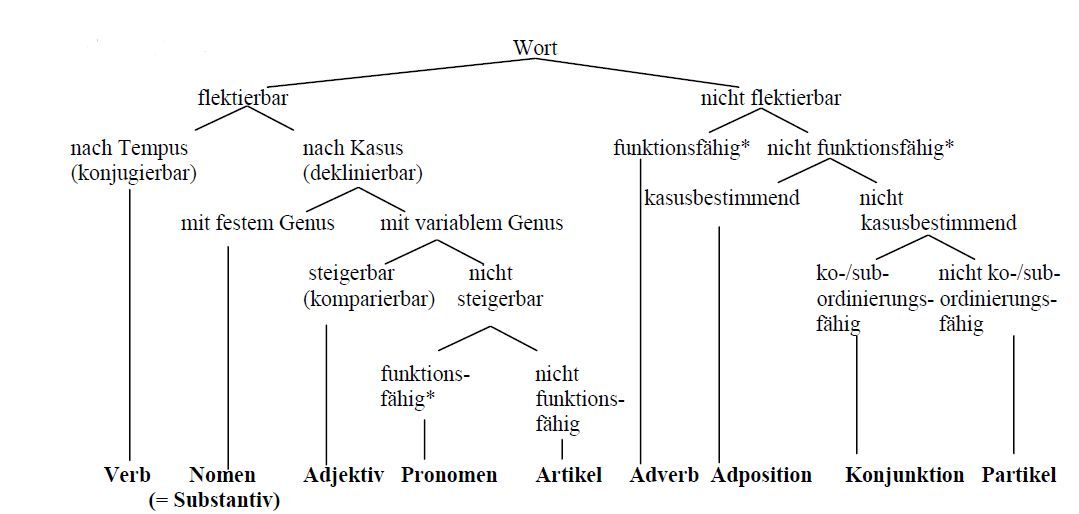
\includegraphics[scale=.4]{material/07wortartenklassifikation}

	
\scalebox{.55}{\begin{forest}MyP edges,
		[Wort
			[flektierbar
				[{nach Tempus\\(konjugierbar)}
				[\textbf{Verb}]
				]
				[{nach Kasus \\(deklinierbar)}
					[{mit festem \\ Genus}
					[{\textbf{Nomen}\\ (\textbf{Substantiv})}]
					]
					[{mit variablem \\Genus}
						[{steigerbar \\(komparierbar)} [\textbf{Adjektiv}] ]
						[{nicht \\steigerbar}
							[funktionsfähig [\textbf{Pronomen}] ]
							[{nicht \\ funktionsfähig} [\textbf{Artikel}] ]
						]
					]
				]
			]
			[{nicht \\flektierbar}
				[funktionsfähig [\textbf{Adverb}] ]
				[{nicht \\funktionsfähig }
					[kasusbestimmend [\textbf{Adposition}] ]
					[{nicht \\kasusbestimmend}
						[{ko-/ \\subordinierungs-\\fähig} [\textbf{Konjunktion}] ]
						[{nicht ko-/ \\ subordinierungs-\\fähig} [\textbf{Partikel}] ]
					]
				]
			]
		]
	\end{forest}}
	\caption{Wortartenklassifikation \citep{Repp&Co15a}}
\end{figure}

\end{frame}


%%%%%%%%%%%%%%%%%%%%%%%%%%%%%%%%%%
\begin{frame}
\frametitle{Wortarten}
\begin{itemize}
	\item \textbf{Schwierigkeiten} mit prototypischen Eigenschaften:

	\eal 
	\ex mithilfe 
	\ex mit Hilfe
	\zl
	
\pause 
Präposition oder Präposition $+$ Nomen ($+$ Nomen im Genitiv?)
\pause

	\ea bausparen 
	\z

\pause	
	nicht V2-fähig wie die \gqq{gewöhnlichen} Verben

\end{itemize}

\end{frame}

%%%%%%%%%%%%%%%%%%%%%%%%%%%%%%%%%%%%%%%

\begin{frame}
\frametitle{Wortarten}

	\begin{itemize}
			\item \textbf{Schwierigkeiten} mit prototypischen Eigenschaften:
				\ea Das \textbf{Schlafen}
			\z
			
			\pause
			Verb oder Nomen?
				\eal
			\ex Er \textbf{kauft} Brot. 
			\ex Er hat das Brot \textbf{gekauft}.
			\pause
			\ex Das \textbf{gekaufte} Brot
			\zl
			
			\pause
			Verb oder Adjektiv?
	\end{itemize}
\end{frame}


%%%%%%%%%%%%%%%%%%%%%%%%%%%%%%%%%%
\begin{frame}
\frametitle{Wortarten}

\begin{itemize}

	\item In unserem Kurs:

\end{itemize}

\begin{table}
\centering
\scalebox{0.9}{
\begin{tabular}{lll}
\textbf{Wortart} & \textbf{Abk.} & \textbf{Beispiel} \\ 
\hline
Nomen (Substantiv) & N & Tisch, Liebe, Maria \\ 
\hline
Determinierer (Artikel, Quantor, Pronomen) & D & der, dem, alle, ein, ich \\ 
\hline
Adjektiv & A & schön, syntaktisch \\ 
\hline
Adverb & Adv & heute, hier \\ 
\hline
Verb & V & rennen, malen \\ 
\hline
Adposition (Prä- \& Postposition) & P & vor, in, wegen, entlang \\ 
\hline
Komplementierer (Subjunktion) & C & ob, dass, weil \\ 
\hline
Konjunktion & K & und, aber, sondern \\ 
\hline
Partikel & Part & ja, wohl, leider \\ 
\hline
\end{tabular} 
}

\end{table}

\end{frame}


%%%%%%%%%%%%%%%%%%%%%%%%%%%%%%%%%%
%%%%%%%%%%%%%%%%%%%%%%%%%%%%%%%%%%
\subsection{Konstituenten}

\iftoggle{sectoc}{
	\frame{
%		\begin{multicols}{2}
		\frametitle{~}
		\tableofcontents[currentsubsection,subsubsectionstyle=hide]
%		\end{multicols}
	}
}


%%%%%%%%%%%%%%%%%%%%%%%%%%%%%%%%%%
\begin{frame}
\frametitle{Konstituenten}

\begin{itemize}
	\item Nicht nur Wörter, sondern auch größere Einheiten spielen in der Syntax eines Satzes eine wichtige Rolle.
	\item Pausen beim Vorlesen:
	\ea Eine 16 Jahre alte Französin starb nach dem Verzehr eines Döners an Lebensmittelvergiftung.\jambox{(Quelle: \url{www.frauenzimmer.de})}
	\z
	
\pause	
	\item Verschiebungen in einem Satz:
	\eal 
	\ex[]{Eine 16 Jahre alte Französin starb \alertred{[nach dem Verzehr]} eines Döners an Lebensmittelvergiftung.}
	\ex[]{\alertred{[Nach dem Verzehr eines Döners]} starb eine 16 Jahre alte Französin an Lebensmittelvergiftung.}
	\ex[*]{\alertred{[Nach dem Verzehr]} starb eine 16 Jahre alte Französin \alertred{[eines Döners]} an Lebensmittelvergiftung.}
	\zl


\end{itemize}

\end{frame}


%%%%%%%%%%%%%%%%%%%%%%%%%%%%%%%%%%
\begin{frame}
\frametitle{Konstituenten}

\begin{itemize}
	\item Wörter bilden (\textbf{konstituieren}) mit anderen Wörtern Konstituenten, die dann gemeinsam größere Konstituenten bilden (vgl.\ Morphologie).
	
	\eal
	\ex{\alertgreen{eines} $+$ [Döners] \pause $=$ \alertred{[eines Döners]}}
	
\pause	
	
	\ex{\alertgreen{Verzehr} $+$ [eines Döners] $=$ \alertred{[Verzehr eines Döners]}}
\pause
	
	\ex{\alertgreen{dem} $+$ [Verzehr eines Döners] $=$ \alertred{[dem Verzehr eines Döners]}}
\pause
	
	\ex{\alertgreen{nach} $+$ [dem Verzehr eines Döners] $=$ \alertred{[nach dem Verzehr eines Döners]}}
	\zl

\end{itemize}

\end{frame}


%%%%%%%%%%%%%%%%%%%%%%%%%%%%%%%%%%
\begin{frame}

\begin{itemize}
	\item Die Gehirnaktivität verdeutlicht die hierarchische Struktur des Satzes (s.\ \citealt{Devitt15a} (pro Chomsky) \vs \citealt{Boutonnet15a} (contra Chomsky)).	
\end{itemize}

\begin{figure}
\centering
%	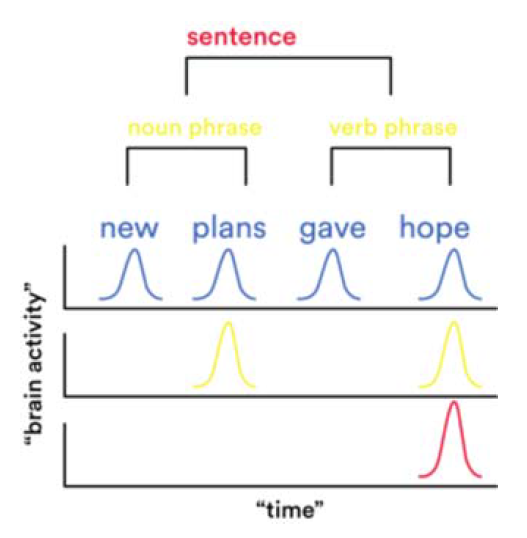
\includegraphics[scale=.33]{material/10gehirnaktivitaet}
	
\begin{tikzpicture}[scale=.48]
	\draw[black](9,0)--(0,0)--(0,1.5);
	\draw[black](9,2)--(0,2)--(0,3.5);
	\draw[black](9,4)--(0,4)--(0,5.5);
	\draw[black](1.5,6.5)--(1.5,7)--(3.5,7)--(3.5,6.5);
	\draw[black](6,6.5)--(6,7)--(8,7)--(8,6.5);
	\draw[black](2.5,8)--(2.5,8.5)--(7,8.5)--(7,8);	
	\node[rotate=90,right] (brain activity) at (-0.6,0) {\scriptsize Gehirnaktivität};
	\node[right] (time) at (2.5,-0.6) {\scriptsize Zeit};
	\node[above] (sentence) at (4.25,8.3) {\scriptsize \alertred{sentence}};
	\node[below] (noun) at (2.5,8) {\scriptsize \alertgreen{noun phrase}};
	\node[below] (verb) at (7,8) {\scriptsize \alertgreen{verbal phrase}};
	\node[below] (new) at (1.5,6.4) {\scriptsize \alertblue{new}};
	\node[below] (plans) at (3.5,6.5) {\scriptsize \alertblue{plans}};
	\node[below] (gave) at (6,6.4) {\scriptsize \alertblue{gave}};
	\node[below] (hope) at (8,6.5) {\scriptsize \alertblue{hope}};	
	\draw[HUblue] (0.75,4.4) sin (1,4.3) cos (1.25,5) sin (1.5,5.5) cos (1.75,5) sin (2,4.3) cos (2.25, 4.4);
	\draw[HUblue] (2.75,4.4) sin (3,4.3) cos (3.25,5) sin (3.5,5.5) cos (3.75,5) sin (4,4.3) cos (4.25, 4.4);
	\draw[HUblue] (5.25,4.4) sin (5.5,4.3) cos (5.75,5) sin (6,5.5) cos (6.25,5) sin (6.5,4.3) cos (6.75, 4.4);
	\draw[HUblue] (7.25,4.4) sin (7.5,4.3) cos (7.75,5) sin (8,5.5) cos (8.25,5) sin (8.5,4.3) cos (8.75,4.4);
	\draw[HUgreen] (7.25,2.4) sin (7.5,2.3) cos (7.75,3) sin (8,3.5) cos (8.25,3) sin (8.5,2.3) cos (8.75,2.4);
	\draw[HUgreen] (2.75,2.4) sin (3,2.3) cos (3.25,3) sin (3.5,3.5) cos (3.75,3) sin (4,2.3) cos (4.25, 2.4);
	\draw[HUred] (7.25,0.4) sin (7.5,0.3) cos (7.75,1) sin (8,1.5) cos (8.25,1) sin (8.5,0.3) cos (8.75,0.4);
\end{tikzpicture}
\caption{\citep[Nach:][]{Boutonnet15a}}
\end{figure}

\end{frame}


%%%%%%%%%%%%%%%%%%%%%%%%%%%%%%%%%%%
\begin{frame}
\frametitle{Konstituenten}

\begin{itemize}
	\item Konstituente: relational zu anderen Konstituenten und zum dem, was sie konstituieren (\ras einfach vs. komplex)
	\medskip
	\item Bei den Konstituenten ist es wichtig herauszufinden, welche sich in Sätzen wie eine \textbf{strukturelle Einheit} verhalten.
	\medskip
	\item In der traditionellen Grammatik \ras Satzglieder und Satzgliedteile

\end{itemize}

\end{frame}


%%%%%%%%%%%%%%%%%%%%%%%%%%%%%%%%%%%
\begin{frame}
\frametitle{Konstituenten}

\begin{itemize}

	\item \textbf{Konstituententests} \citep[vgl.][]{MyP18a}
	\begin{itemize}
		\item Ersetzungstest (oder Substitutionstest)
		\item Pronominalisierungstest
		\item Fragetest
		\item Verschiebetest (oder Permutationstest)
		\item Vorfeldtest (oder Voranstellungstest) 
		\item Weglasstest (oder Eliminierungstest)
		\item (Koordinationstest, Parenthesetest, \dots )
	\end{itemize}
	\medskip
	\item (Phrasale) Konstituenten sollten sich \textbf{in den meisten} dieser Tests \textbf{als syntaktische Einheit verhalten}.

\end{itemize}

\end{frame}


%%%%%%%%%%%%%%%%%%%%%%%%%%%%%%%%%%%
%%%%%%%%%%%%%%%%%%%%%%%%%%%%%%%%%%
\subsubsection{Ersetzungstest}

%\iftoggle{sectoc}{
%	\frame{
%		\begin{multicols}{2}
%		\frametitle{~}
%		\tableofcontents[currentsubsection,subsubsectionstyle=hide]
%		\end{multicols}
%	}
%}

%%%%%%%%%%%%%%%%%%%%%%%%%%%%%%%%%%%
\begin{frame}
\frametitle{Ersetzungstest (Substitutionstest)}

\begin{itemize}
	\item Was sich durch ein anderes Wort (/""eine andere Wortfolge) ersetzen lässt, so dass der Satz grammatisch bleibt, ist (vermutlich) eine (phrasale) Konstituente.

	\eal 
	\ex[]{\alertred{[Eine Frau]} starb nach dem Verzehr eines Döners.}
	\ex[]{\alertred{[Ein Mann]} starb nach dem Verzehr eines Döners.}
	\ex[*]{\alertred{[Ein Mann]} nach dem Verzehr eines Döners.}
	\zl

\pause	
	\eal 
	\ex Die Frau hat versucht, \alertred{[den Döner zu genießen]}.
	\ex Die Frau hat versucht, \alertred{[uns allen Weihnachtsgeschenke zu geben]}.
	\zl
	
\end{itemize}

\nocite{MyP18m}

\end{frame}


%%%%%%%%%%%%%%%%%%%%%%%%%%%%%%%%%%%
%%%%%%%%%%%%%%%%%%%%%%%%%%%%%%%%%%
\subsubsection{Pronominalisierungstest}

%\iftoggle{sectoc}{
%	\frame{
%		\begin{multicols}{2}
%		\frametitle{~}
%		\tableofcontents[currentsubsection,subsubsectionstyle=hide]
%		\end{multicols}
%	}
%}

%%%%%%%%%%%%%%%%%%%%%%%%%%%%%%%%%%%
\begin{frame}
\frametitle{Pronominalisierungstest}

\begin{itemize}
	\item Unterart des Ersetzungstests
	\medskip
	\item Was sich durch ein Pronomen ersetzen lässt, so dass der Satz grammatisch bleibt, ist (vermutlich) eine (phrasale) Konstituente.

	\eal 
	\ex[]{\alertred{[Eine Frau]} starb \alertred{[nach dem Verzehr eines Döners]}.}
	\ex[]{\alertred{[Sie]} starb \alertred{[dann]}.}
	\ex[*]{\alertred{[Sie]} nach dem Verzehr eines Döners.}
	\ex[*]{Eine Frau \alertred{[dann]}.}
	\zl

\pause	
	\eal 
	\ex Die Frau versucht, \alertred{[den Döner zu genießen]}.
	\ex Die Frau versucht \alertred{[das]}.
	\zl
	
\end{itemize}

\end{frame}


%%%%%%%%%%%%%%%%%%%%%%%%%%%%%%%%%%%
%%%%%%%%%%%%%%%%%%%%%%%%%%%%%%%%%%
\subsubsection{Fragetest}

%\iftoggle{sectoc}{
%	\frame{
%		\begin{multicols}{2}
%		\frametitle{~}
%		\tableofcontents[currentsubsection,subsubsectionstyle=hide]
%		\end{multicols}
%	}
%}

%%%%%%%%%%%%%%%%%%%%%%%%%%%%%%%%%%%
\begin{frame}
\frametitle{Fragetest}

\begin{itemize}
	\item Unterart des Ersetzungstests
	\medskip
	\item Was sich erfragen lässt (durch ein W-Wort ersetzen lässt), so dass der Satz grammatisch bleibt, ist (vermutlich) eine (phrasale) Konstituente.

	\eal 
	\ex[]{\alertred{[Eine Frau]} starb \alertred{[nach dem Verzehr eines Döners]}.}
	\ex[]{\alertred{[Wer]} starb nach dem Verzehr eines Döners?}
	\ex[]{\alertred{[Wann]} starb eine Frau?}
	\ex[*]{\alertred{[Wer]} nach dem Verzehr eines Döners?}
	\ex[*]{\alertred{[Wann]} eine Frau?}
	\zl

\pause	
	\eal 
	\ex Die Frau versucht, \alertred{[den Döner zu genießen]}.
	\ex \alertred{[Was]} versucht die Frau?
	\zl
	
\end{itemize}

\nocite{MyP18j}

\end{frame}


%%%%%%%%%%%%%%%%%%%%%%%%%%%%%%%%%%%
%%%%%%%%%%%%%%%%%%%%%%%%%%%%%%%%%%
\subsubsection{Verschiebetest}


%\iftoggle{sectoc}{
%	\frame{
%		\begin{multicols}{2}
%		\frametitle{~}
%		\tableofcontents[currentsubsection,subsubsectionstyle=hide]
%		\end{multicols}
%	}
%}

%%%%%%%%%%%%%%%%%%%%%%%%%%%%%%%%%%%
\begin{frame}
\frametitle{Verschiebetest (Permutationstest)}

\begin{itemize}
	\item Was sich innerhalb des Satzes verschieben lässt, so dass der Satz grammatisch bleibt, ist (vermutlich) eine (phrasale) Konstituente.

	\eal 
	\ex[]{Nach dem Verzehr eines Döners starb \alertred{[gestern]} \alertred{[eine Frau]}.}
	\ex[]{Nach dem Verzehr eines Döners starb \alertred{[eine Frau]} \alertred{[gestern]}.}
	\ex[*]{Nach dem Verzehr eines Döners starb \alertred{[eine]} [gestern] [Frau].}
	\zl

\pause	
	\eal 
	\ex Die Frau hat noch nicht versucht, \alertred{[den Döner zu genießen]}.
	\ex Die Frau hat \alertred{[den Döner zu genießen]} noch nicht versucht.
	\ex Die Frau hat noch nicht \alertred{[den Döner zu genießen]} versucht.
	\zl

\end{itemize}

\nocite{MyP18l}

\end{frame}


%%%%%%%%%%%%%%%%%%%%%%%%%%%%%%%%%%%
%%%%%%%%%%%%%%%%%%%%%%%%%%%%%%%%%%
\subsubsection{Vorfeldtest}

%\iftoggle{sectoc}{
%	\frame{
%		\begin{multicols}{2}
%		\frametitle{~}
%		\tableofcontents[currentsubsection,subsubsectionstyle=hide]
%		\end{multicols}
%	}
%}


%%%%%%%%%%%%%%%%%%%%%%%%%%%%%%%%%%%
\begin{frame}
\frametitle{Vorfeldtest (Voranstellungstest)}

\begin{itemize}
	\item Unterart des Verschiebetests
	\medskip
	\item Im Deutschen kann vor dem finiten Verb nur eine Konstituente stehen. 
	\medskip
	\item Was sich in einem Aussagesatz vor das finite Verb verschieben lässt, so dass der Satz grammatisch bleibt, ist (vermutlich) eine (phrasale) Konstituente.

\end{itemize}

\end{frame}


%%%%%%%%%%%%%%%%%%%%%%%%%%%%%%%%%%%
\begin{frame}
\frametitle{Vorfeldtest (Voranstellungstest)}

\begin{itemize}
	\item Was sich in einem Aussagesatz vor das finite Verb verschieben lässt, so dass der Satz grammatisch bleibt, ist (vermutlich) eine (phrasale) Konstituente.

	\eal
	\ex[]{\alertred{[Nach dem Verzehr eines Döners]} starb [gestern] [eine Frau].}
	\ex[]{\alertred{[Gestern]} starb [eine Frau] [nach dem Verzehr eines Döners].}
	\ex[]{\alertred{[Eine Frau]} starb [gestern] [nach dem Verzehr eines Döners].}
	\ex[*]{\alertred{[Nach]} starb [eine Frau] [gestern] \alertred{[dem Verzehr eines Döners]}.}
	\ex[*]{\alertred{[Eine]} starb \alertred{[Frau]} [gestern] [nach dem Verzehr eines Döners].}
	\ex[*]{\alertred{[Eines Döners]} starb [eine Frau] [gestern] [nach dem Verzehr].}
	\zl

\end{itemize}

\end{frame}


%%%%%%%%%%%%%%%%%%%%%%%%%%%%%%%%%%%
\begin{frame}
\frametitle{Vorfeldtest (Voranstellungstest)}

\begin{itemize}
	\item Was sich in einem Aussagesatz vor das finite Verb verschieben lässt, so dass der Satz grammatisch bleibt, ist (vermutlich) eine (phrasale) Konstituente.

	\eal 
	\ex[]{Die Frau hat noch nicht versucht, \alertred{[den Döner zu genießen]}.}
	\ex[]{\alertred{[Den Döner zu genießen]} hat die Frau noch nicht versucht.}
	\ex[]{\alertred{[Auf den Döner warten]} wollte er nicht mehr.}
	\ex[*]{\alertred{[den Döner]} wollte er nicht mehr auf warten.}
	\zl

\end{itemize}

\end{frame}


%%%%%%%%%%%%%%%%%%%%%%%%%%%%%%%%%%%
%%%%%%%%%%%%%%%%%%%%%%%%%%%%%%%%%%
\subsubsection{Weglasstest}

%\iftoggle{sectoc}{
%	\frame{
%		\begin{multicols}{2}
%		\frametitle{~}
%		\tableofcontents[currentsubsection,subsubsectionstyle=hide]
%		\end{multicols}
%	}
%}

%%%%%%%%%%%%%%%%%%%%%%%%%%%%%%%%%%%
\begin{frame}
\frametitle{Weglasstest (Eliminierungstest)}

\begin{itemize}
	\item Was sich in elliptischen Konstruktionen weglassen lässt, so dass der Satz grammatisch bleibt, ist (vermutlich) eine (phrasale) Konstituente.

	\eal 
	\ex[]{Maria liebt \sout{[Knoblauchsoße]} und Peter hasst \alertred{[Knoblauchsoße]}.}
	\ex[]{Maria chillt \sout{[an einem sonnigen Tag]} und schreibt Lieder \alertred{[an einem sonnigen Tag]}.}
	\ex[*]{Maria chillt \sout{[an einem]} \alertred{sonnigen Tag} und schreibt Lieder \alertred{[an einem sonnigen Tag]}.}
	\zl

\end{itemize}

\nocite{MyP18f}

\end{frame}


%%%%%%%%%%%%%%%%%%%%%%%%%%%%%%%%%%
%%%%%%%%%%%%%%%%%%%%%%%%%%%%%%%%%%
\subsection{Hausaufgabe}
%\frame{
%\frametitle{~}
%	\tableofcontents[currentsection]
%}
%%%%%%%%%%%%%%%%%%%%%%%%%%%%%%%%%%

%%%%%%%%%%%%%%%%%%%%


\begin{frame}
\frametitle{Hausaufgabe}

\begin{itemize}
	\item Geben Sie die Wortart der folgenden Einheiten an:
\end{itemize}

\begin{columns}
\column{.30\textwidth}
	\begin{enumerate}
	\item Maria
	\item Ach!
	\item kauft
	\item den
	\item an
	\item weil
	\item beachten
	\item obwohl
	\end{enumerate}

\column{.50\textwidth}

\end{columns}

\end{frame}


\iftoggle{ha-loesung}{


%%%%%%%%%%%%%%%%%%%%%%%%%%%%%%%%%%

} 
%%%%%%%%%%%%%%%%%%%%



%%%%%%%%%%%%%%%%%%%%%%%%%%%%%%%%%%
\begin{frame}
\frametitle{Hausaufgabe}

\begin{itemize}
	\item Testen Sie mithilfe von mindestens zwei Konstituententests, ob die fettgedruckten Wortfolgen eine oder mehrere Konstituenten sind.
\end{itemize}

	\ea Maria \textbf{stolperte über} den Stein.

	\ex Der Minister wird in \textbf{der nächsten Woche} die Aussage wiederholen.
	
	\ex Die Besucher beobachteten \textbf{in der Werkstatt bemaltes Porzellan}.
	
	\ex Die Besucher beobachteten \textbf{in der Werkstatt} bemaltes Porzellan.
		
	\ex Erika traf die \textbf{Lehrerin mit den roten Schuhen}.
	
	\ex Helmut hat sehr lange \textbf{auf Maria gewartet}.
	
	\ex Helmut hat sehr lange \textbf{auf Maria} gewartet.
	
	\ex \textbf{Maria wird} nach diesem Kurs Syntax lieben.
	\z
	
\end{frame}
	
%%%%%%%%%%%%%%%%%%%%
\iftoggle{ha-loesung}{
	
	%%%%%%%%%%%%%%%%%%%%%%%%%%%%%%%%
%06b Syntax ha-loesung
%%%%%%%%%%%%%%%%%%%%%%%%%%%%%%


\begin{frame}
\frametitle{Hausaufgabe -- Lösung}

\begin{itemize}
	\item Geben Sie die Wortart der folgenden Einheiten an:
\end{itemize}

\begin{columns}
	\column{.30\textwidth}
	\begin{enumerate}
		\item Maria
		\item Ach!
		\item kauft
		\item den
		\item an
		\item weil
		\item beachten
		\item obwohl
	\end{enumerate}
	
	\column{.50\textwidth}

\pause
	
	\begin{enumerate}
		\item[\ras] \alertgreen{Nomen (Substantiv)}
		\item[\ras] \alertgreen{Interjektion}
		\item[\ras] \alertgreen{Verb}
		\item[\ras] \alertgreen{Determinierer}
		\item[\ras] \alertgreen{Präposition}
		\item[\ras] \alertgreen{Complementizer/Subjunktion}
		\item[\ras] \alertgreen{Verb}
		\item[\ras] \alertgreen{Complementizer/Subjunktion}
	\end{enumerate}
\end{columns}

\end{frame}
	
	
	%%%%%%%%%%%%%%%%%%%%%%%%%%%%%%%%%%
	\begin{frame}
	\frametitle{Hausaufgabe -- Lösung}
	
	
	\begin{itemize}
		\item Testen Sie mithilfe von mindestens zwei Konstituententests, ob die fettgedruckten Wortfolgen eine oder mehrere Konstituenten sind.
		
		\vspace{.5cm}
		
		\item[] Maria \textbf{stolperte über} den Stein.
	\end{itemize}
	
	\pause 
	
	\ea Weglasstest \& Fragetest \ras \alertgreen{keine Konstituente}
	\ea[*]{Maria [stolperte über] den Stein und Peter [\sout{stolperte über}] den Ast.}
	\ex[*]{[Was] Maria den Stein?}
	\z 
	\z
	
\end{frame}


%%%%%%%%%%%%%%%%%%%%%%%%%%%%%%%%%%
\begin{frame}
\frametitle{Hausaufgabe -- Lösung}

\begin{itemize}
\item[] Der Minister wird in \textbf{der nächsten Woche} die Aussage wiederholen.
\end{itemize}

\pause 

\ea Ersetzungstest, Koordinationstest, Fragetest, Vorfeldtest \ras \alertgreen{keine Konstituente}

\ea[??]{Der Minister wird in [dieser] die Aussage wiederholen.}
\ex[?]{Der Minister wird in [der nächsten Woche] und [dem nächsten Treffen] die Aussage wiederholen.}
\ex[*]{[Wann] wird der Minister in die Aussage wiederholen?}
\ex[*]{[Der nächsten Woche] wird der Minister in die Aussage wiederholen.}
\z 
\z

\end{frame}


%%%%%%%%%%%%%%%%%%%%%%%%%%%%%%%%%%
\begin{frame}
\frametitle{Hausaufgabe -- Lösung}

\begin{itemize}
\item[] Die Besucher beobachteten \textbf{in der Werkstatt bemaltes Porzellan}.

\item[] Die Besucher beobachteten \textbf{in der Werkstatt} bemaltes Porzellan.
\end{itemize}

\pause 

\ea Vorfeldtest, Pronominalisierungstest \ras \alertgreen{1 Konstituente} 
\ea {[}In der Werkstatt bemaltes Porzellan{]} beobachteten die Besucher.
\ex Die Besucher beobachteten [es].
\z 

\pause 

\ex Verschiebetest, Pronominalisierungstest, Fragetests \ras \alertgreen{2 Konstituenten}
\ea Die Besucher beobachteten [bemaltes Porzellan] [in der Werkstatt]. 
\ex Die Besucher beobachteten [es] [dort].
\ex {[}Was{]} beobachteten die Besucher [in der Werkstatt]?
\ex {[}Wo{]} beobachteten die Besucher [bemaltes Porzellan]?
\z
\z

\end{frame}


%%%%%%%%%%%%%%%%%%%%%%%%%%%%%%%%%%%%%%%%%%%%%%%%%%%%%%%

\begin{frame}
\frametitle{Hausaufgabe -- Lösung}

\begin{itemize}
\item[] Erika traf die \textbf{Lehrerin mit den roten Schuhen}.
\end{itemize}

\pause 

\ea Weglasstest, Vorfeldtest, Fragetest \ras \alertgreen{keine Konstituente}
\ea[*]{Erika traf die und begrüßte die [Lehrerin mit den roten Schuhen].}
\ex[*]{[Lehrerin mit den roten Schuhen] traf Erika die.}
\ex[*]{[Wen] traf Erika die?}
\z 
\z
\end{frame}


%%%%%%%%%%%%%%%%%%%%%%%%%%%%%%%%%%%%%%%%%%%%%%%%%%%%%%%

\begin{frame}
\frametitle{Hausaufgabe -- Lösung}

\begin{itemize}
\item[] Helmut hat sehr lange \textbf{auf Maria gewartet}.

\item[] Helmut hat sehr lange \textbf{auf Maria} gewartet.
\end{itemize}

\pause 

\ea Vorfeldtest, Fragetest, Verschiebetest \ras \alertgreen{1 aber auch 2 Konstituenten}
\ea[]{[Auf Maria gewartet] hat Helmut sehr lange.}
\ex[]{[Was] hat Helmut sehr lange?}
\ex[??]{Helmut hat [auf Maria gewartet] sehr lange.}
\ex[]{Helmut hat [auf Maria] sehr lange [gewartet].}
\ex[]{[Auf Maria] hat Helmut sehr lange gewartet.} 
\z
\z 

\end{frame}


%%%%%%%%%%%%%%%%%%%%%%%%%%%%%%%%%%%%%%%%%%%%%%%%%%%%%%

\begin{frame}
\frametitle{Hausaufgabe -- Lösung}

\begin{itemize}
\item[] \textbf{Maria wird} nach diesem Kurs Syntax lieben.
\end{itemize}

\pause 

\ea Verschiebetest, Fragetest, Weglasstest \ras \alertgreen{keine Konstituente}
\ea[*]{Nach diesem Kurs [Maria wird] Syntax lieben.}
\ex[*]{[Wer] nach diesem Semester Syntax lieben?}
\ex[]{[Maria wird] nach diesem Kurs Syntax lieben und [\sout{Maria wird}] nur noch an Bäume denken.}
\z 
\z

\end{frame}
	
} 
%%%%%%%%%%%%%%%%%%%%


%%%%%%%%%%%%%%%%%%%%%%%%%%%%%%%%%%
\subsection{Sonstiges}
%\frame{
%\frametitle{~}
%	\tableofcontents[currentsection]
%}


%%%%%%%%%%%%%%%%%%%%%%%%%%%%%%%%%%
\begin{frame}
\frametitle{Was Sie sich zu Weihnachten wünschen können\dots}

\begin{itemize}
	\item \citet{Glueck&Roedel16a} (auch über die HU-Bibliothek herunterladbar)
	\item \citet{Luedeling2009a}
	\item \citet{Brandt&Co06a}
	\item \citet{Grewendorf&Co91a}
	\item \citet{Chomsky65a}
	\item \citet{MuellerS15b} (auch über die Webseite herunterladbar)
	\item \citet{MuellerS13f} (auch über die Webseite herunterladbar)
	\item \citet{Pinker95a}

\end{itemize}

\end{frame}


%%%%%%%%%%%%%%%%%%%%%%%%%%%%%%%%%%
\begin{frame}
\frametitle{Frohe Weihnachten!}

\begin{figure}
\centering
\scalebox{.7}{
	\begin{forest}MyP edges,
[TP
	[DP [\zerobar{D} [\textcolor{orange}{\textbf{this}} ] ] ]
	[\MyPxbar{T}
		[\zerobar{T} [\textcolor{violet}{\textbf{is\textsubscript{i}}}] ]
		[VP 
			[\zerobar{V} [\textcolor{blue}{\textbf{t\textsubscript{i}}}] ]
			[DP
				[\zerobar{D} [\textcolor{magenta}{\textbf{my}}] ]
				[NP
				[AP [\zerobar{A} [\textcolor{red}{\textbf{christmas}} ] ] ]
					[\zerobar{N} [\textcolor{green}{\textbf{tree}}] ]
				]
			]
		]
	]
]
\end{forest}
}
\caption{Weihnachtsbaum}
\end{figure}
%\begin{figure}
%\centering
%	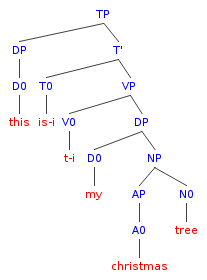
\includegraphics[scale=.57]{material/09xmastree}
%	\caption{Frohe Weihnachten!}
%\end{figure}

\end{frame}

%%%%%%%%%%%%%%%%%%%%%%%%%%%%%%%%%%

\subsection{Abbildungen}
\begin{frame}{Abbildungen}
\small

\begin{itemize}
	\item ABBILDUNG -- \gqq{Noam Chomsky. Aufgenommen von John Soares, 2005} (Stevertigo, Zugriff: 18.07.2018) \url{https://upload.wikimedia.org/wikipedia/commons/8/86/Noam_chomsky.jpg}
	\item ABBILDUNG -- \gqq{Schimpansenfamilie} (Stock-Foto, Zugriff: 18.07.2018) \url{https://www.colourbox.de/bild/familie-auf-der-oberseite-des-baumes-bild-2566359}
\end{itemize}	

\end{frame}
